\documentclass[conference]{IEEEtran}
%\hyphenation{op-tical net-works semi-conduc-tor}
\usepackage[bibstyle=ieee, citestyle=numeric-comp]{biblatex}
\usepackage{graphicx}
\usepackage{amsmath}
\usepackage{listings}
\usepackage{caption}
\usepackage{subcaption}
\usepackage{csquotes}
\usepackage{float}
\usepackage{color}
\usepackage{gensymb}
\usepackage{multirow}
\usepackage{array}
\usepackage{mathtools}
\usepackage[thinlines]{easytable}
\DeclarePairedDelimiter{\abs}{\lvert}{\rvert}
\usepackage[toc,page]{appendix}
\usepackage{setspace}
\usepackage{biblatex}
\addbibresource{ref.bib}
\captionsetup[figure]{labelfont={bf},labelformat={default},labelsep=period,name={Fig.}}
\addbibresource{ref.bib}
\renewcommand\IEEEkeywordsname{Keywords}

\begin{document}

\title{Suspicious Bangla Text Detection Using\\ Machine Learning}

\author{\IEEEauthorblockN{\textbf{Omar Sharif}}
\IEEEauthorblockA{Dept. of Computer Science \& Engineering\\
Chittagong University of Engineering and Technology\\
Chittagong-4349, Bangladesh\\
Email: omar.shaif1303@gmail.com}
\and
\IEEEauthorblockN{\textbf{Mohammed Moshiul Hoque}}
\IEEEauthorblockA{Professor, Department of CSE\\
Chittagong University of Engineering and Technology\\
Chittagong-4349, Bangladesh\\
Email: moshiulh@yahoo.com}}


\maketitle

%%%%%%% Abstract and Keyword section %%%%%%%
%%%%%%%%%%%%%%%%%%%%%%%%%%%%%%%%%%%%%%%%%%%%
\begin{abstract}
Suspicious Bangla text detection is a text classification problem of classifying Bangla text into suspicious and non suspicious category. In this paper we tried to find out the  performance of different statistical machine learning algorithm for detecting suspicious Bangla text. To the best of our knowledge, it is very first work on detecting suspicious Bangla text so we have to develop a corpus of suspicious Bangla text. This paper shows comparison of accuracy of different machine learning algorithm which will be helpful to others. The experimental result shows maximum accuracy of 92\% for Logistic Regression using 1500 training documents and 500 testing documents. The overall accuracy can be increased by increasing number of text documents in the dataset and considering semantic relation between words of a sentence.  
\end{abstract}
\vspace{0.3cm}
\begin{IEEEkeywords}
 Suspicious Bangla text, Text classification, Text classification methods, Bangla language processing, Machine learning. 
\end{IEEEkeywords}

\IEEEpeerreviewmaketitle

%%%%%%%%%% Introduction %%%%%%%%%%%%%%%%%%%%
%%%%%%%%%%%%%%%%%%%%%%%%%%%%%%%%%%%%%%%%%%%%
\section{Introduction}
Text classification is the task of assigning a text document into a set of predefined classes in an intelligent manner. Because of the rapid growth of online information, text classification has become more challenging and more important as well. Digitization has changed
the way we process and analyze information. There is an exponential increase in online availability of information. From web pages to emails, science journals, ebooks, learning content, news and social media are all full of textual data. Text classification performs an essential role in various applications that deals with organizing, classifying, searching and concisely representing a significant amount of information. Detecting suspicious text is typically a text classification problem where we have to classify a text as suspicious and not suspicious. Suspicious text detection is a kind of system where suspicious texts are identified by the keywords used in the text body. As most of our communications are text based, if we able to predict either a text is suspicious or not suspicious it will be very helpful for our law enforcement agencies to find the perpetrator and stop terrorist event. As far we know, no system is developed for detecting suspicious Bangla text. It is very important for the safety of Bangladeshi People to develop a system which can detect suspicious communications in Bangla. This motivated us to work in this area.

In this work, our original purpose is to develop a framework for detecting suspicious Bangla texts using supervised machine learning techniques. In this paper, we have applied Naïve Bayes Classifier\cite{yoo2015classification}, Support Vector Machine\cite{wei2012text, villmann2017can}, Logistic regression\cite{sharma2015active}, K-nearest neighbor algorithms (KNN)\cite{harisinghaney2014text}, Decision Trees\cite{chavan2014survey} to detect suspicious Bangla text and also find out the accuracy of this algorithms.

%%%%%%%%%% Related Work %%%%%%%%%%%%%%%%%%%%
%%%%%%%%%%%%%%%%%%%%%%%%%%%%%%%%%%%%%%%%%%%%
\section{\textbf{Related Work}}
A number of significant researches have already done in text classification in English and other language. Major works of text classification are Email classification, Research paper categorization, Detecting suspicious profiles etc.
But research on Bangla text classification is in preliminary stage still now. However some mentionable works have been done for Bangla Language Processing.
\vspace{0.2cm}

Hossain et al. describes Bengali document categorization based on word embedding and statistical learning approaches\cite{hossain2018automatic}. It categorizes document into nine predefined categories with mentionable accuracy. An Arabic text categorization system is developed using Naive Bayes in control environment dataset with good accuracy\cite{alsaleem2011automated}.
Krendzelak et al. describe a system which categorize text with machine learning and hierarchical structures by using tree based Naive Bayesian categorization process\cite{krendzelak2015text, chy2014bangla}. It performs with low accuracy due to training techniques and training feature extraction process.
\vspace{0.2cm}

S. Alami et al. describes about different techniques to detect suspicious profiles using text analysis within social media\cite{alami2015detecting}. A system for detecting suspicious email using enhanced feature selection is proposed but it has low accuracy because of not having enough dataset\cite{nizamani2013modeling}. Text Categorization of Turkish language using SVM is proposed which achieved better accuracy but due to large feature dimensions time complexity is large\cite{kaya2012sentiment}. Better result can be obtained by using clustering based approach \cite{ismail2014bangla, ahmad2016bengali} but a lot of problem exist with cluster-based solution. In our work, a system is developed and trained with different machine learning algorithms and overall accuracy of this algorithms is measured over our dataset.

%%%%%%%%% Methodology %%%%%%%%%%%%%%%%%%%%%%
%%%%%%%%%%%%%%%%%%%%%%%%%%%%%%%%%%%%%%%%%%%%
\section{\textbf{Methodology}}
The key objective of our project is to design a system that can classify suspicious and non-suspicious text. \textbf{Fig} \ref{fig:proposed_model} shows an abstract view of our suspicious text detector classifier.

\begin{figure}[h!]
\centering
  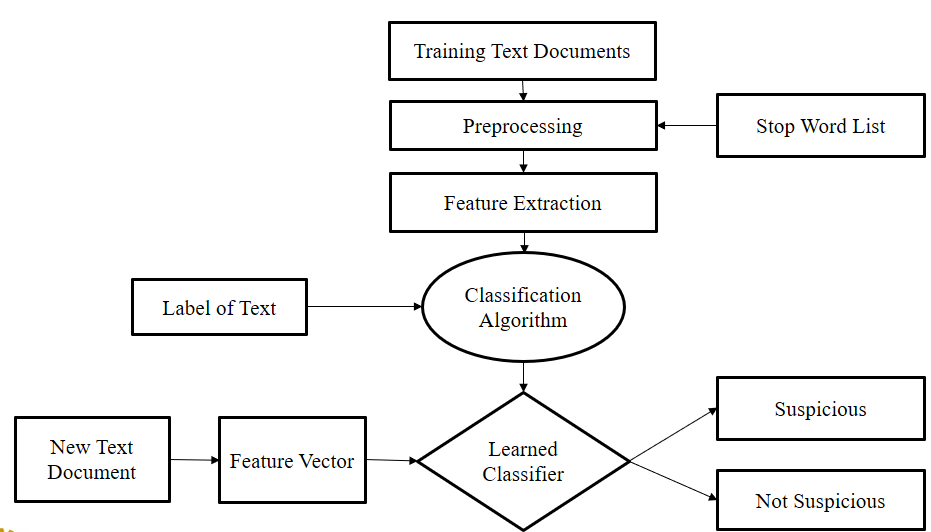
\includegraphics[scale=0.365]{Figures/proposed_model.PNG}
  \caption{ Model for Suspicious Text Detection}
  \label{fig:proposed_model}
\end{figure}

We have implemented this system by using different supervised machine learning algorithms. As a supervised classification problem, our whole system is classified into two phases one is training phase and another is testing phase.
\subsection{\textbf {Training Phase}}
In training set each document is labeled as either suspicious or non suspicious. Training phase of suspicious text detector includes five steps:
\subsubsection{\textbf{Training Set Preparation}}
Training set is divided into positive set (suspicious texts) and negative set (non suspicious texts).
\subsubsection{\textbf{Text Preprocessing}}
All texts are preprocessed by the preprocessor in order to remove inconsistencies for dataset. In our system the word which has no contribution in deciding whether a text is suspicious or not suspicious is referred as stop word. Such words are removed form the text by matching with a stop word list. 
\subsubsection{\textbf{Feature Extraction}}
A word list is created by the tokenizer by tokenizing the main body of a text. Word frequencies is used as features in this system. Bag of words model is used to represent the features. Our feature space is a two dimensional array where rows represents each text of the corpus and columns represents unique words available in the corpus. Each cell of the array represents the number of time a specific word occurs in a specific text.
\subsubsection{\textbf{Training the Suspicious Text Detector}}
It is most important part of our whole system. If we able to train our model correctly than the output will be better. Five different machine learning algorithms is used to train our model. 
\vspace{0.3cm}

\textbf{Naive Bayes}\cite{yoo2015classification} can be defined as Bayes theorem with a conditional independency assumption that all variables $A_{1},A_{2},...,A_{n}$ in a given category $C$ are conditionally independent with each other given $C$. 
According to Bayes rule for a text document $(T)$ and class $(C)$ we can write,
\begin{equation}
    P(C|T) = \frac{P(T|C)P(C)}{P(T)}
\end{equation}
The class we are looking for to assign this document is out of all classes the one that maximizes the probability of that class given the document.
\begin{equation}\label{eq:11}
 \begin{aligned}
     C_{MAP} & = argmax P(C|T) \\     & = argmax \frac{P(T|C)P(C)}{P(T)}
\end{aligned}
\end{equation}
So final equation for Naive Bayes Classifier is,
\begin{equation}
     C_{MAP} = argmax P(X_{1},X_{2},...,X_{n}|C)P(C)
\end{equation}
\vspace{0.1cm}

\textbf{SVM}\cite{wei2012text} analyze data used for classification and regression analysis. SVM can perform linear classification as well as non-linear classification using kernel trick. For linear classification cost function can be written as,
\begin{equation}
    \label{cost_function_svm}
    \frac{1}{n}\sum_{i=1}^{n}\max{(0,1-y_{i}(w.x_{i}-b))} + \lambda (\lVert \mathbf{w} \rVert)^2
\end{equation}
The parameter $\lambda $ in above equation determines the trade-off between increasing the margin-size and ensuring that the samples lie on the correct side of the margin.

For non-linear classification with SVM kernel trick is used. Some common kernel tricks used in machine learning are,
\begin{itemize}
    \item Gaussian radial basis function:
    \begin{equation}
         k(x_{i}, x_{j}) = \exp{(-\gamma(\lVert \mathbf{x_{i}-x_{j}} \rVert)^2)}
    \end{equation}
    \item Polynomial Kernel (homogeneous):
    \begin{equation}
        k(x_{i}, x_{j}) = (x_{i}\cdot x_{j})^d
    \end{equation}
     \item Polynomial Kernel (inhomogeneous):
     \begin{equation}
         k(x_{i}, x_{j}) = (x_{i}\cdot x_{j}+1)^d
     \end{equation}
\end{itemize}
\vspace{0.1cm}

A \textbf{Decision Tree}\cite{chavan2014survey} has two types of nodes one is external and another is internal. Decision classes are represented by external node of a decision tree. Internal nodes corresponds to attribute which are used for making decision by decision tree algorithm. Decision tree is simple to build and as it is a inductive algorithm it can be interpreted easily. Entropy is used to calculate the homogeneity of a sample. To build a decision tree, we need to calculate two types of entropy using as follows,
\begin{enumerate}
    \item Entropy using one attribute :
    \begin{equation}
         E(S) = \sum_{i=1}^{c}-P_i \log_2P_i
    \end{equation}
    \item Entropy using two attributes :
    \begin{equation}
        E(S) = \sum_{c\epsilon X}{}P(C)E(C) 
    \end{equation}
    
\end{enumerate}


\textbf{Logistic Regression}\cite{sharma2015active} is a binary classification model that predicts a binary outcome based on some features. The output of logistic regression depends on logistic function. The definition of logistic function or hypothesis function is,
\begin{equation}
    h_{\theta}(x) =  \frac{1}{1+\exp({-\theta^T x})}
\end{equation}
Cost function for Logistic regression is,
\begin{equation}
    J(\theta) = \frac{1}{m}\sum_{i-1}^{m}cost(h_{\theta}(x^{i}),y^{i})   
\end{equation}

\[
cost(h_{\theta}(x), y) = 
\begin{cases}
    -\log (h_{\theta}(x)) & \texttt{if } y = 1\\
     -\log (1-h_{\theta}(x)) & \texttt{if } y = 0
\end{cases}
\]
Here,\\
$m = $ Number of training examples.\\
$h_{\theta}(x^{i}) = $ Hypothesis function of $i_{th}$ training example\\
$y^i = $ Input label of $i_{th}$ training example.

\vspace{0.3cm}

\textbf{KNN}\cite{harisinghaney2014text} is a non-parametric method used for
classification and regression. K nearest neighbors is a simple algorithm that stores all available cases and classifies new cases based on a similarity measure (e.g., distance functions). Most commonly used three different distance function of K-NN are,

\begin{enumerate}
    \item Euclidean distance function :
    \begin{equation}
        \sqrt{\sum_{i=1}^{k}(x_i-y_i)^2}
    \end{equation}
    \item Manhattan distance function :
    \begin{equation}
         \sum_{i=1}^{k}\abs{(x_i-y_i)}
    \end{equation}
    \item Minkowski distance function :
    \begin{equation}
        ({\sum_{i=1}^{k}(\abs{x_i-y_i})^q)})^\frac{1}{q}
    \end{equation}
    
\end{enumerate}
All three distance measures are only valid for continuous variables.

\subsubsection{\textbf{Saving the Model}}
The result of the training phase is used in testing phase. The result is saved as a model which contains knowledge for classifying a new text document into suspicious or non suspicious category.

\subsection{\textbf{Testing Phase}}
Testing is the most important phase for any machine learning model. Classification accuracy of the text classifier is calculated in testing phase. In our system testing phase is quite similar as training phase but in this part our learned classifier model is used for predicting. Sample texts are taken to test the system. After processing, using feature extraction methods features are extracted from the texts. Our classifier model use this features to classify a text as suspicious and non suspicious.

%%%%%%%%% Experiments %%%%%%%%%%%%%%%%%%%%%%
%%%%%%%%%%%%%%%%%%%%%%%%%%%%%%%%%%%%%%%%%%%%
\section{Experiments}
For the successful implementation of any machine learning algorithm dataset is the key. It was a very challenging task for us to build a corpus which contains a large amount of suspicious and non suspicious text. We have collected non suspicious data from a pre-build corpus\cite{banglacorpus}, thanks to them. Suspicious data are collected from different online and offline resources.% Data stored in .txt format.
\par \vspace{0.3cm} 
We mark a text as suspicious if it has one of the following features,
\begin{itemize}
    \item Texts contain words which hurts our religious feelings.\vspace{0.2cm} 
    \item Texts which instigate people against government.\vspace{0.2cm} 
    \item Texts which instigate people against law enforcement agencies.\vspace{0.2cm} 
    \item Texts which motivate people in terrorist events.\vspace{0.2cm} 
    \item Texts which instigate a community without any reason.\vspace{0.2cm} 
    \item Texts which instigate our political parties. 
\end{itemize}
 \par \vspace{0.3cm}
 Most of our suspicious data about religion are collected from online blogs\cite{nastikya, dhormo, istishon}. Suspicious data about politics is collected from websites of different newspaper\cite{palo, kk, juga}. Data is also collected from different public pages of Facebook\cite{bash}. Table \ref{data} represents the statistics of data used for our model.
 
 \renewcommand{\arraystretch}{1.3}
\begin{table}[h!]
\begin{center}
\caption{Data Summary}
\begin{tabular}{|m{4.8cm} | m{3cm}|}
\hline
     Number of training documents & 1500 \\
\hline
     Number of testing documents & 500 \\
\hline
     Number of sentences & 8991\\
\hline 
     Number of words & 35964\\
\hline 
     Total unique words & 4295\\
\hline
\end{tabular}
\label{data}
\end{center}
\end{table}

In order to classify the texts, we have fed our collected documents to our classifier model. As dataset is collected manually it may have some inconsistency.

%%%%%%%% Evaluation Measures %%%%%%%%%%%%%%%
%%%%%%%%%%%%%%%%%%%%%%%%%%%%%%%%%%%%%%%%%%%%
\section{\textbf{Evaluation Measures}}
To evaluate our proposed system we used several statistical measures such as Confusion matrix, Precision, Recall, F$_1$ score and graphical measures such as Precision-Recall curve, Receiver Operating Characteristics (ROC) curve.
\subsection{\textbf{Confusion Matrix}}
A confusion matrix is a table that is used to evaluate the performance of a classification model. As ours is a binary classification model, the confusion matrix of our system has two rows and two columns. This matrix reports the number of false positives, false negatives, true positives, and true negatives.
\par
\vspace{0.3cm}
\noindent
\textbf{Fig.} \ref{fig:CM} shows confusion matrix for our system.\clearpage
\begin{figure}[h!]
    \centering
    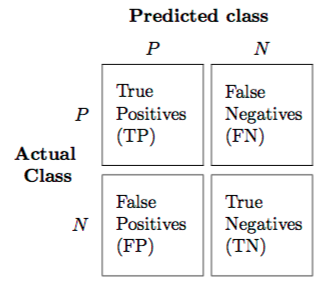
\includegraphics[scale=0.50]{Figures/confusion_matrix_1.png}
    \caption{Confusion Matrix}
    \label{fig:CM}
\end{figure}
\begin{itemize}
    \item True Positive(TP): Number of documents that is suspicious and also classified as suspicious.\vspace{0.2cm}
    \item True Negative(TN): Number of documents that is non suspicious and also classified as non suspicious.\vspace{0.2cm}
    \item False Negative(FN): Number of documents that is suspicious but classified as non suspicious.\vspace{0.2cm}
    \item False Positive(FP): Number of documents that is non suspicious but classified as suspicious. 
\end{itemize}
\noindent
This numbers are used to calculate other evaluation measures.

\subsection{\textbf{Precision}}
Precision refers as positive predictive value. That is the ratio of correctly classified positive instances to the total number of instances classified as positive. Precision can be obtained form  the following equation.
\begin{equation}
    \texttt{Precision} = \frac{TP}{TP+FP}
\end{equation}
If precision is high then the algorithm is doing well.

\subsection{\textbf{Recall}}
Recall is the ratio of correctly classified positive instances to the total number of positive instances. It is also called true positive rate. Recall can be obtained from the following equation.
\begin{equation}
    \texttt{Recall} = \frac{TP}{TP+FN}
\end{equation}
High precision and high Recall is essential for a model.

\subsection{\textbf{$F_1$ score}}
 $F_1$ score is the weighted average of Precision and Recall. To chose a learning algorithm between several algorithms we have to find $F_1$ Score of algorithms. F1-score can be obtained from the following equation,
 \begin{equation}
     F_1 = \frac{2*precision*recall}{precision+recall}
 \end{equation}
$F_1$ score is usually more useful than accuracy

\subsection{\textbf{Precision Recall Curve}}
Precision Recall curves summarize the trade-off between the true positive rate and the positive predictive value for a predictive model using different probability thresholds. A precision-recall curve is a plot of the precision (y-axis) and the recall (x-axis) for different thresholds.

\subsection{\textbf{ROC Curve}}
Receiver Operating Characteristic (ROC) curves summarize the trade-off between the true positive rate and false positive rate for a predictive model using different probability thresholds.%ROC curves are appropriate when the observations are balanced between each class. 
It is a plot of the false positive rate (x-axis) versus the true positive rate (y-axis) for a number of different candidate threshold values between 0 and 1.

%%%%%%% Experimental Results %%%%%%%%%%%%%%
%%%%%%%%%%%%%%%%%%%%%%%%%%%%%%%%%%%%%%%%%%%
\section{\textbf{Experimental Results}}
Table \ref{AE} represents accuracy and error rate of different classification algorithm on our dataset.
\renewcommand{\arraystretch}{1.5}
\begin{table}[h!]
\begin{center}
\caption{Evaluation Summary}
\begin{tabular}{|m{4.5cm} | m{1.6cm}| m{1.6cm}|}
\hline
     Classification Algorithm & Accuracy  & Error  \\
\hline
    Naive Bayes & 0.85 & 0.15\\
\hline 
    SVM (Linaer Kernel) & 0.91 & 0.09\\
\hline 
    SVM (RBF Kernel) & 0.90 & 0.10\\
\hline 
    Logistic Regression & 0.92 & 0.08\\
\hline
    K-Nearest Neighbor & 0.73 & 0.27\\
\hline
    Decision Tree & 0.88 & 0.12\\
\hline
\end{tabular}
\label{AE}
\end{center}
\end{table}
\par
Table \ref{prr} shows the precision, recall and $F_1$ score of different classification algorithm used in our model.

\begin{table}[h!]
\begin{center}
\caption{Performance Comparison}
\begin{tabular}{|m{3.6cm} | m{1.25cm}| m{1.2cm}| m{1.3cm}|}
\hline
     Classification Algorithm & Precision & Recall & $F_1$ score \\
\hline
    Naive Bayes & 0.89 & 0.85 & 0.85\\
\hline 
    SVM (Linaer Kernel) & 0.91 & 0.91 & 0.91\\
\hline 
    SVM (RBF Kernel) & 0.90 & 0.91 & 0.90\\
\hline 
    Logistic Regression & 0.91 & 0.93 & 0.93\\
\hline
    K-Nearest Neighbor & 0.82 & 0.73 & 0.70\\
\hline
    Decision Tree & 0.88 & 0.92 & 0.89\\
\hline
\end{tabular}
\label{prr}
\end{center}
\end{table}

For all of the algorithms we use similar number of training and test documents. From table \ref{AE} and \ref{prr}, we can see that Logistic Regression and Support Vector Machine algorithm's are performing up to the mark on our dataset. Naive Bayes and Decision tree also doing really well. But accuracy of K-nearest neighbour is really poor compare to other algorithms. 

Now, we will learn about classification report, Precision Recall curve and Receiver operating characteristic's (ROC) curve of  all of this algorithms. Classification report gives us precision, recall and $F_1$ score of each category which is really helpful to analyze the algorithm.
\subsection{\textbf{Naive Bayes Classifier}}
Table \ref{NBC} shows the classification report and \textbf{Fig.} \ref{prrn} shows Precision-Recall and ROC curve for Naive Bayes classifier.  .
\renewcommand{\arraystretch}{1.2}
\begin{table}[h!]
\begin{center}
\caption{Classification Report (Naive Bayes)}
\begin{tabular}{|m{2.8cm} | m{1.5cm}| m{1.3cm}| m{1.5cm}|}
\hline
     & Precision & Recall & $F_1$ score\\
\hline
     Suspicious & 1.00 & 0.71 & 0.83\\
\hline 
     Non suspicious  & 0.76 & 1.00 & 0.87\\
\hline 
     avg./total & 0.89 & 0.85 & 0.85\\
\hline
\end{tabular}
\label{NBC}
\end{center}
\end{table}

\begin{figure}[H]
\centering
\subcaptionbox{Precision Recall}{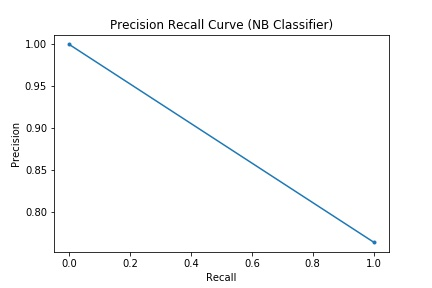
\includegraphics[scale=0.29]{Figures/PRN.jpg}}%
\hfill % <-- Seperation
\subcaptionbox{ROC}{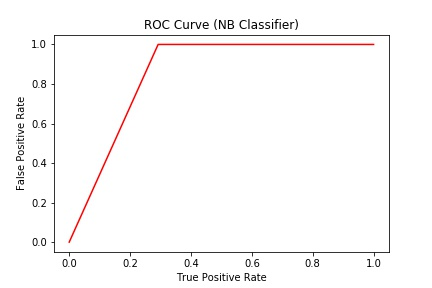
\includegraphics[scale =0.29]{Figures/ROCN.jpg}}%
\caption{Result of Naive Bayes Classifier}
\label{prrn}
\end{figure}


\subsection{\textbf{SVM (Linear Kernel)}}
Table \ref{SVML} shows the classification report and \textbf{Fig.} \ref{slk} shows Precision-Recall and ROC curve for Support Vector Machine with linear kernel.

\begin{table}[h!]
\begin{center}
\caption{Classification Report (SVM Linear Kernel)}
\begin{tabular}{|m{2.8cm} | m{1.5cm}| m{1.3cm}| m{1.5cm}|}
\hline
     & Precision & Recall & $F_1$ score\\
\hline
     Suspicious & 0.91 & 1.00 & 0.91\\
\hline 
     Non suspicious  & 1.00 & 0.90 & 0.91\\
\hline 
     avg./total & 0.91 & 0.91 & 0.91\\
\hline
\end{tabular}
\label{SVML}
\end{center}
\end{table}

\begin{figure}[H]
\centering
\subcaptionbox{Precision Recall}{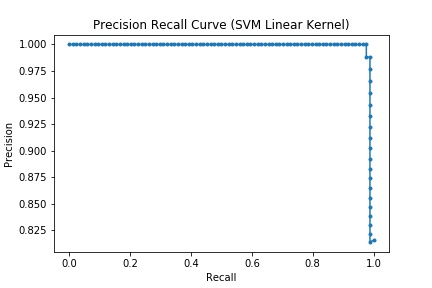
\includegraphics[scale=0.29]{Figures/PRSL.jpg}}%
\hfill % <-- Seperation
\subcaptionbox{ROC}{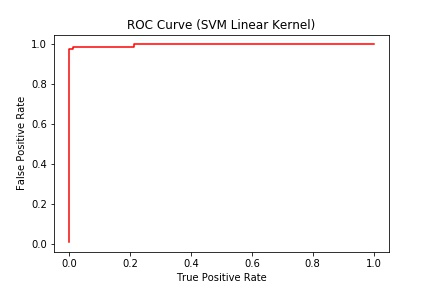
\includegraphics[scale =0.29]{Figures/ROCSL.jpg}}%
\caption{Result of SVM (Linear Kernel)}
\label{slk}
\end{figure}

\subsection{\textbf{SVM (RBF Kernel)}}
Results of Support Vector Machine with RBF kernel are shown in table \ref{SVMR} and \textbf{Fig.} \ref{svr}.
\renewcommand{\arraystretch}{1.1}
\begin{table}[h!]
\begin{center}
\caption{Classification Report (SVM RBF Kernel)}
\begin{tabular}{|m{2.8cm} | m{1.5cm}| m{1.3cm}| m{1.5cm}|}
\hline
     & Precision & Recall & $F_1$ score\\
\hline
     Suspicious & 0.90 & 0.99 & 0.90\\
\hline 
     Non suspicious  & 0.99 & 0.89 & 0.91\\
\hline 
     avg./total & 0.90 & 0.91 & 0.90\\
\hline
\end{tabular}
\label{SVMR}
\end{center}
\end{table}

\begin{figure}[H]
\centering
\subcaptionbox{Precision Recall}{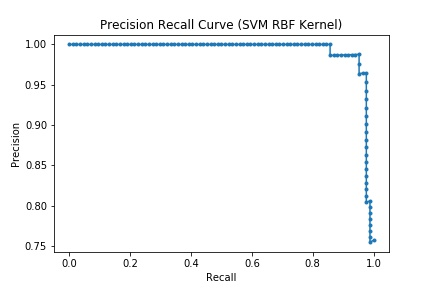
\includegraphics[scale=0.29]{Figures/PRSR.jpg}}%
\hfill % <-- Seperation
\subcaptionbox{ROC}{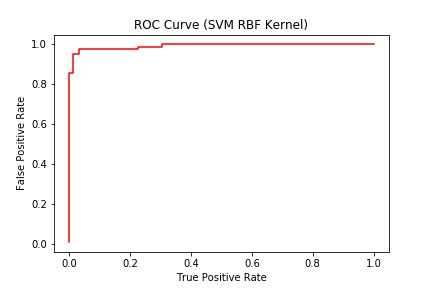
\includegraphics[scale =0.29]{Figures/ROCSR.jpg}}%
\caption{Result of SVM (RBF Kernel)}
\label{svr}
\end{figure}

\subsection{\textbf{Logistic Regression}}
Results of Logistic Regression classifier are shown in table \ref{lr} and \textbf{Fig.} \ref{flr}.

\begin{table}[h!]
\begin{center}
\caption{Classification Report (Logistic Regression)}
\begin{tabular}{|m{2.8cm} | m{1.5cm}| m{1.3cm}| m{1.5cm}|}
\hline
     & Precision & Recall & $F_1$ score\\
\hline
     Suspicious & 0.92 & 1.00 & 0.93\\
\hline 
     Non suspicious  & 1.00 & 0.93 & 0.93\\
\hline 
     avg./total & 0.91 & 0.93 & 0.93\\
\hline
\end{tabular}
\label{lr}
\end{center}
\end{table}

\begin{figure}[H]
\centering
\subcaptionbox{Precision Recall}{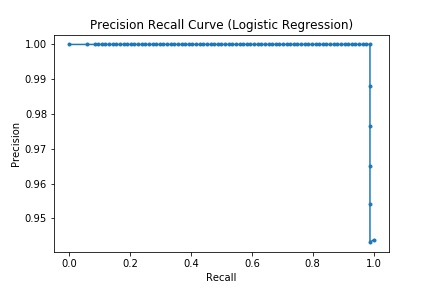
\includegraphics[scale=0.29]{Figures/PRLR.jpg}}%
\hfill % <-- Seperation
\subcaptionbox{ROC}{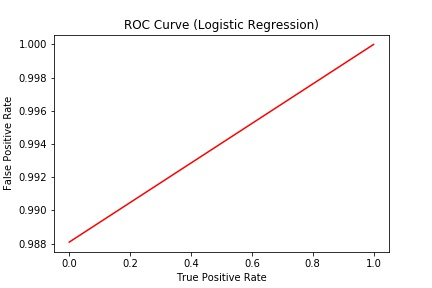
\includegraphics[scale =0.29]{Figures/ROCLR.jpg}}%
\caption{Result of Logistic Regression}
\label{flr}
\end{figure}



\subsection{\textbf{K-Nearest Neighbor}}
\renewcommand{\arraystretch}{1}
\begin{table}[h!]
\begin{center}
\caption{Classification Report (K-Nearest Neighbor)}
\begin{tabular}{|m{2.8cm} | m{1.5cm}| m{1.3cm}| m{1.5cm}|}
\hline
     & Precision & Recall & $F_1$ score\\
\hline
     Suspicious & 0.65 & 1.00 & 0.79\\
\hline 
     Non suspicious  & 1.00 & 0.44 & 0.61\\
\hline 
     avg./total & 0.82 & 0.73 & 0.70\\
\hline
\end{tabular}
\label{tknn}
\end{center}
\end{table}


\begin{figure}[H]
\centering
\subcaptionbox{Precision Recall}{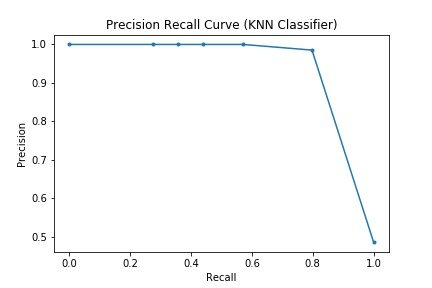
\includegraphics[scale=0.29]{Figures/PRKNN.jpg}}%
\hfill % <-- Seperation
\subcaptionbox{ROC}{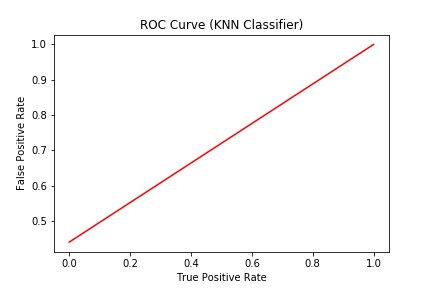
\includegraphics[scale =0.29]{Figures/ROCKNN.jpg}}%
\caption{Result of K-Nearest Neighbor}
\label{fknn}
\end{figure}

\subsection{\textbf{Decision Tree}}

Results of Decision Tree classifier are shown in table \ref{tdct} and \textbf{Fig.} \ref{fdct}.

\begin{table}[h!]
\begin{center}
\caption{Classification Report (Decision Tree)}
\begin{tabular}{|m{2.8cm} | m{1.5cm}| m{1.3cm}| m{1.5cm}|}
\hline
     & Precision & Recall & $F_1$ score\\
\hline
     Suspicious & 0.91 & 0.89 & 0.90\\
\hline 
     Non suspicious  & 0.88 & 0.90 & 0.89\\
\hline 
     avg./total & 0.90 & 0.90 & 0.90\\
\hline
\end{tabular}
\label{tdct}
\end{center}
\end{table}

\begin{figure}[H]
\centering
\subcaptionbox{Precision Recall}{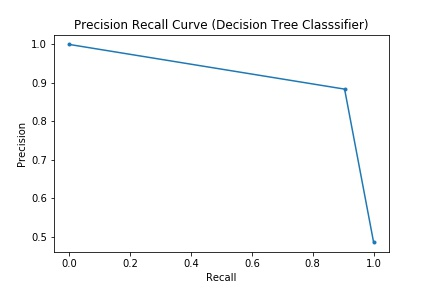
\includegraphics[scale=0.29]{Figures/PRDCT.jpg}}%
\hfill % <-- Seperation
\subcaptionbox{ROC}{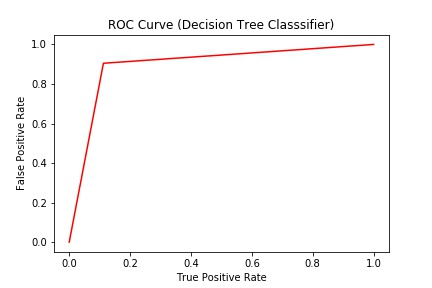
\includegraphics[scale =0.29]{Figures/ROCDCT.jpg}}%
\caption{Result of Decision Tree}
\label{fdct}
\end{figure}


%%%% Conclusion and Future Improvement %%%%
%%%%%%%%%%%%%%%%%%%%%%%%%%%%%%%%%%%%%%%%%%%
\section{\textbf{Conclusion and Future Improvement}}


\renewcommand{\bibfont}{\normalfont\small}
\printbibliography

\end{document}


